\begin{frame}

\end{frame}

\begin{frame}{数式に頼らない「レオロジー超入門講座」}

\begin{block}{東亞合成(株)}

\end{block}

\begin{block}{佐々木裕}

\end{block}

\end{frame}

\begin{frame}{1\_はじめに}

\begin{itemize}

\item
  簡単な自己紹介
\item
  レオロジーとは
\item
  難しい点
\item
  理解へのアプローチ
\item
  本講座の進め方
\end{itemize}

\end{frame}

\begin{frame}

\begin{block}{簡単な自己紹介}

\begin{itemize}

\item
  自己紹介

  \begin{itemize}
  
  \item
    佐々木裕
  \item
    東亞合成(株) 1986~現在
  \end{itemize}
\item
  研究・開発歴

  \begin{itemize}
  
  \item
    各種の光硬化型材料
  \item
    機能性材料の特性評価
  \item
    シミュレーションやレオロジー
  \end{itemize}
\item
  モットー

  \begin{itemize}
  
  \item
    化学をベースに、尤もらしく。\\
  \item
    物理、数学、統計の考えを利用して。
  \end{itemize}
\end{itemize}

\end{block}

\end{frame}

\begin{frame}

\begin{block}{レオロジーとは}

\end{block}

\end{frame}

\begin{frame}

\begin{block}{レオロジーとは}

1929年にアメリカにおいてレオロジー学会\\
「 The Society of Rheology (SOR) 」が設立された。

aaaa

\href{fig/fig_4_3/N1_Melt.mp4}{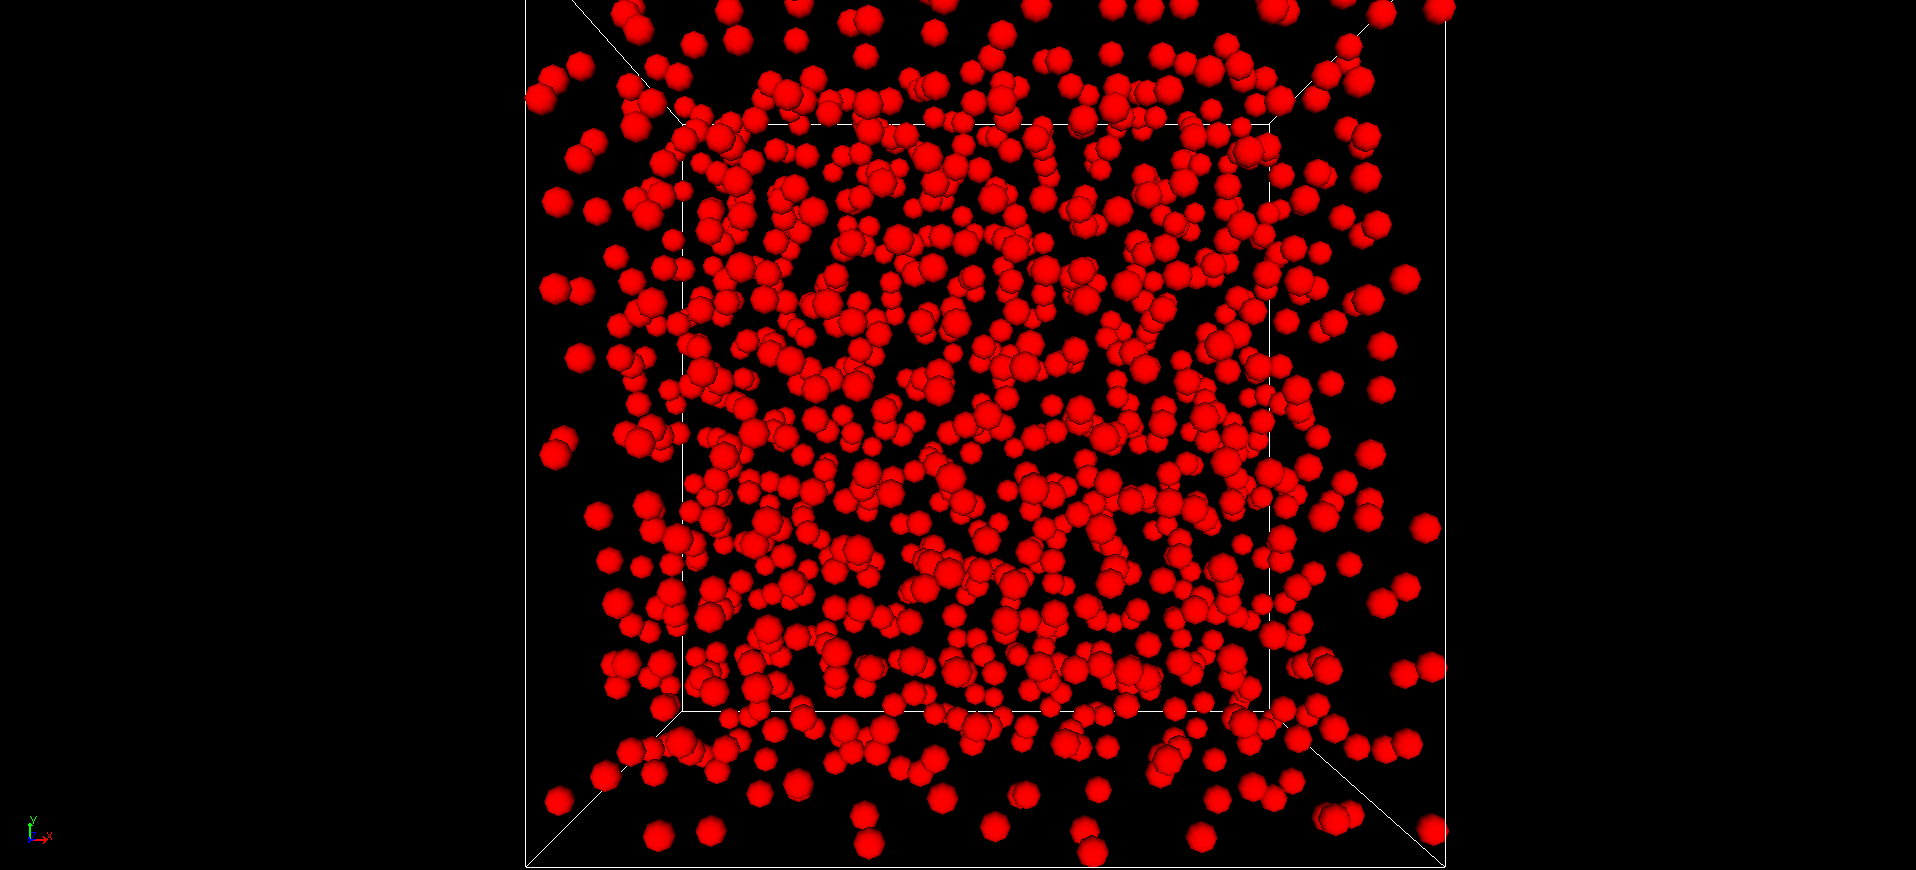
\includegraphics{fig/fig_4_3/N1_Melt.png}}

\end{block}

\end{frame}

\begin{frame}

\begin{block}{相対的な比較(異種格闘技?)}

\begin{itemize}

\item
  水と蜂蜜の力学的性質を比べるとずいぶん違う

  \begin{itemize}
  
  \item
    蜂蜜

    \begin{itemize}
    
    \item
      容易にかき回すことができない。
    \item
      流れにくい。
    \end{itemize}
  \item
    水

    \begin{itemize}
    
    \item
      たやすくコップに注ぎ込むことができる。
    \end{itemize}
  \end{itemize}
\item
  このちがいを何であらわすか?
\item
  例えば、ハチミツとマヨネーズでは?
\end{itemize}

\end{block}

\end{frame}

\begin{frame}

\begin{block}{レオロジーとは}

\begin{itemize}

\item
  現象論的には、以下の三つの関係を調べ、物質の特性を評価する科学。
\end{itemize}

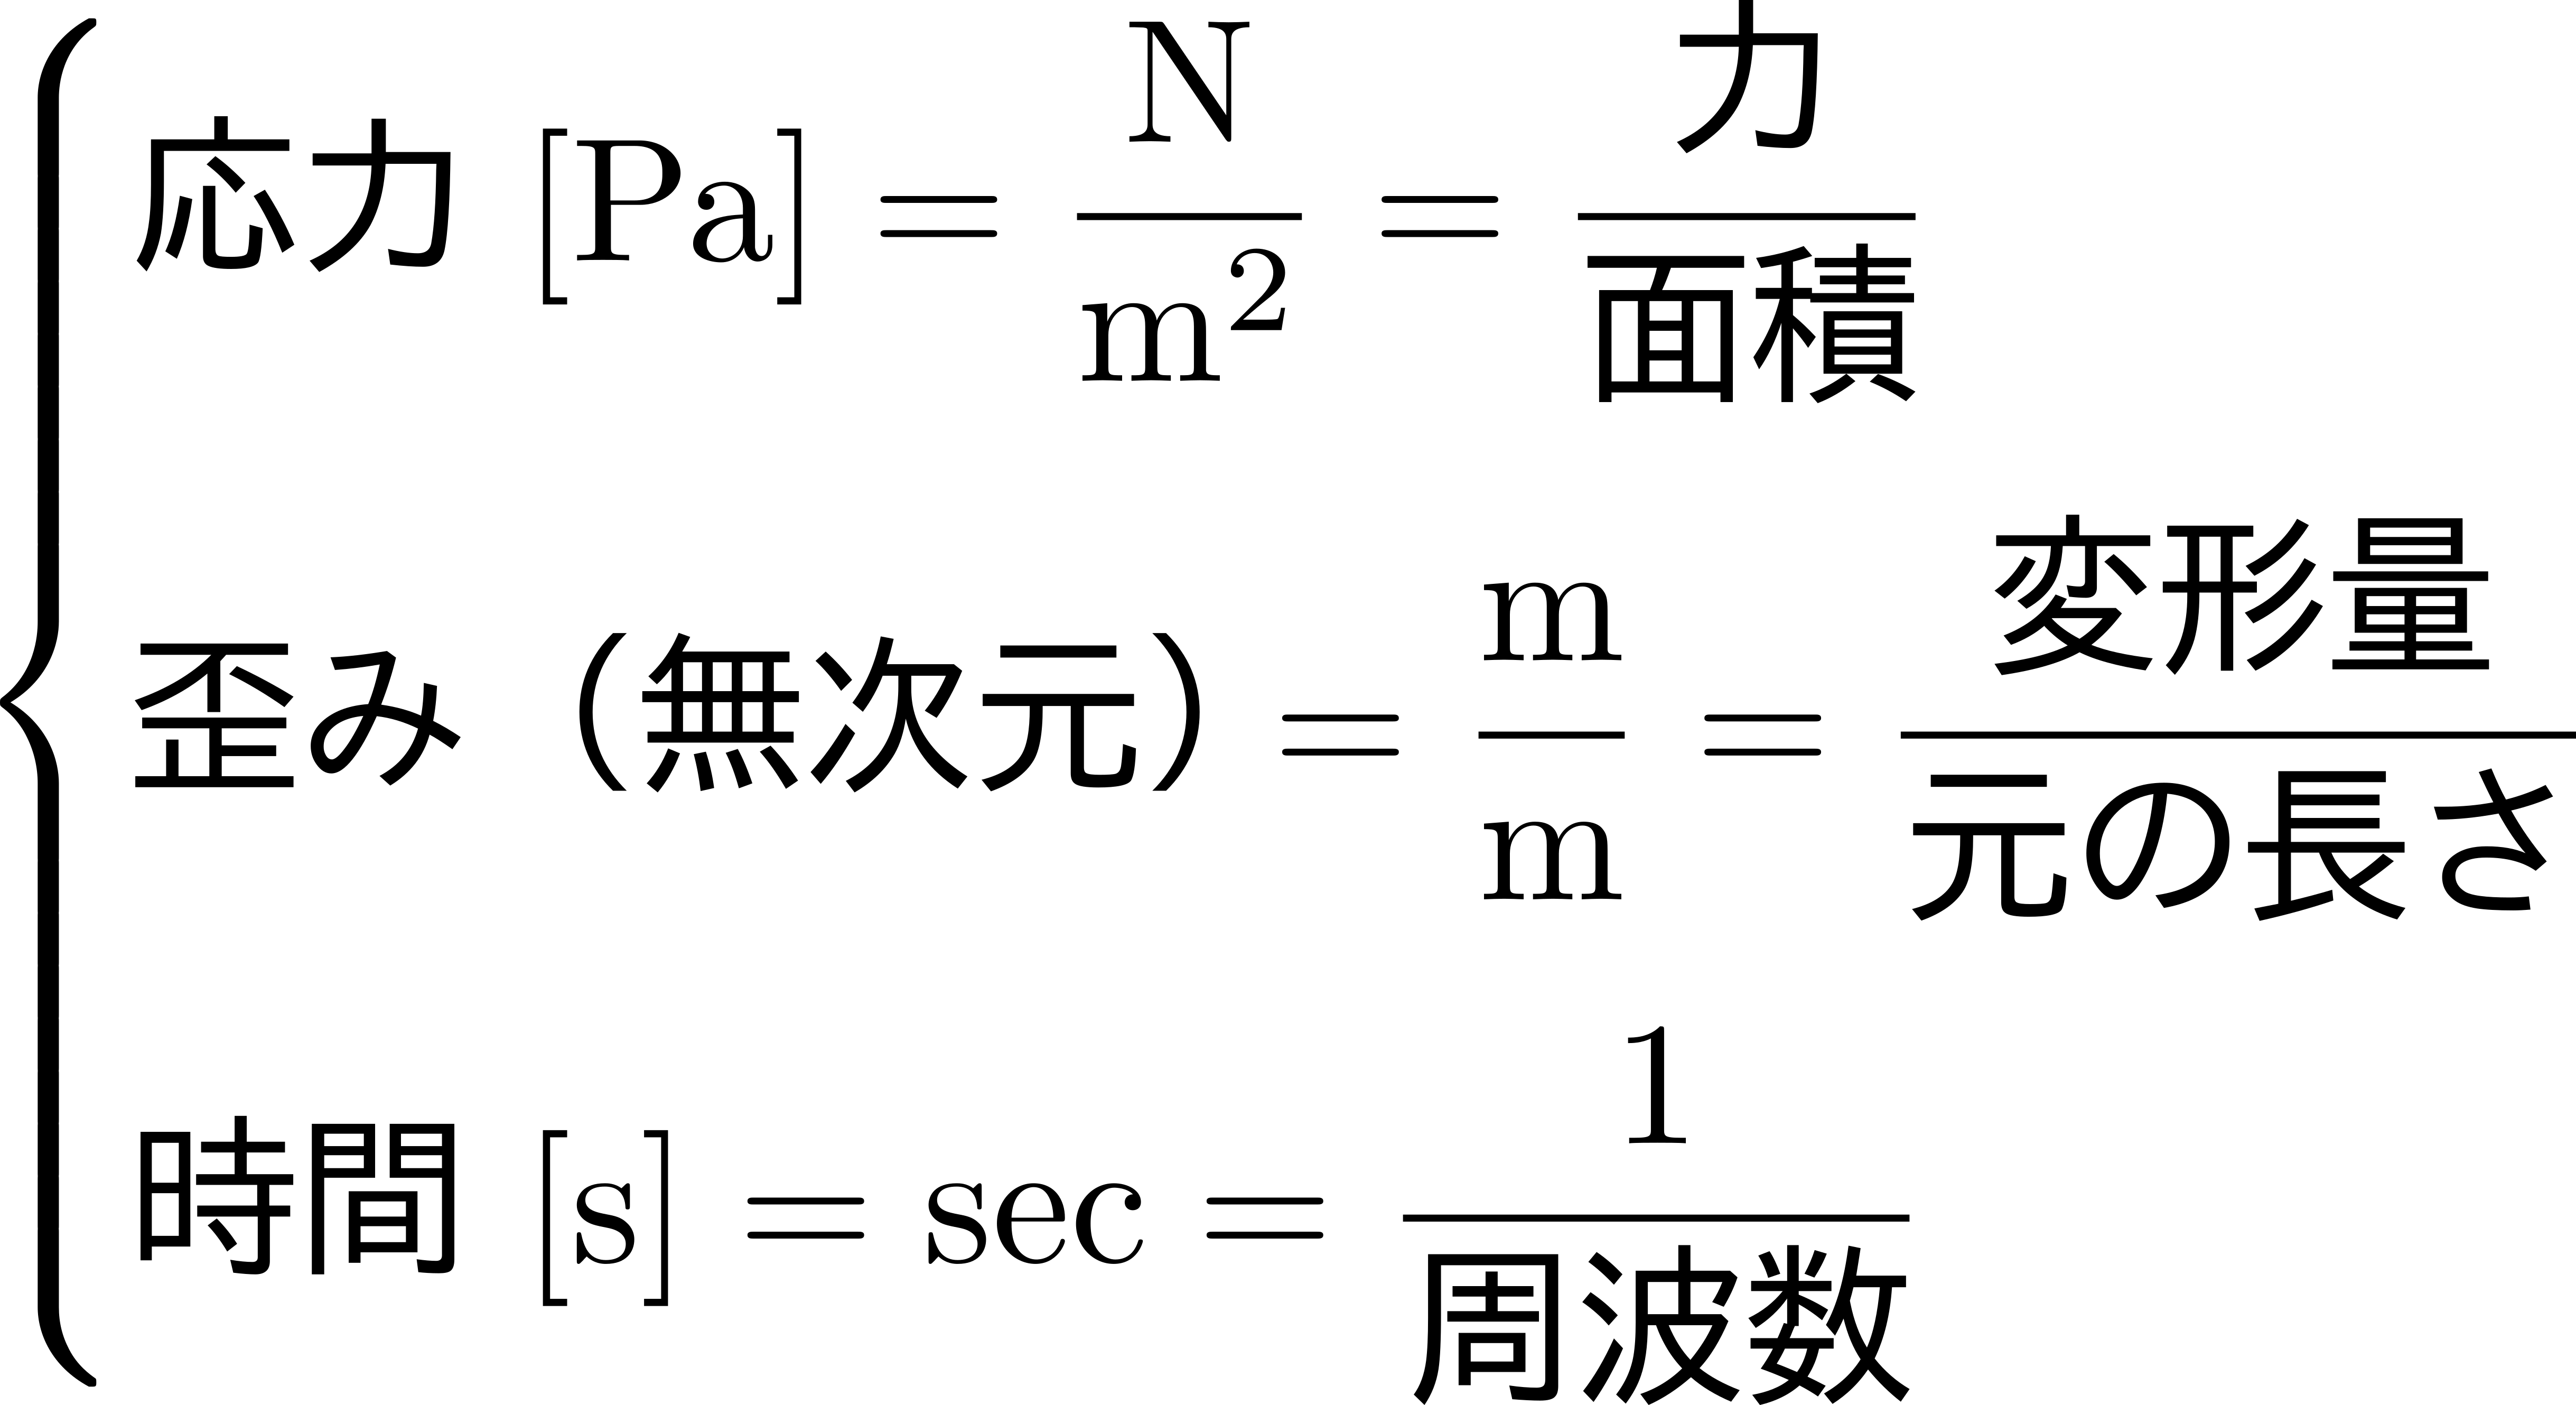
\includegraphics{fig/fig_1/レオロジーの関係.png}

\end{block}

\end{frame}

\begin{frame}

\begin{block}{難しい点}

\end{block}

\end{frame}

\begin{frame}

\begin{block}{両極端な議論}

\begin{itemize}

\item
  あまりにもイメージに偏った議論

  \begin{itemize}
  
  \item
    この時はこう、あの時はああ。
  \item
    それなら。今はどの時?
  \end{itemize}
\item
  分かり難い言葉と数式の羅列で数学的なお話

  \begin{itemize}
  
  \item
    例えば、一般化マックスウェルモデルの動的貯蔵弾性率を表す数式
  \end{itemize}
\end{itemize}

\begin{figure}
\centering
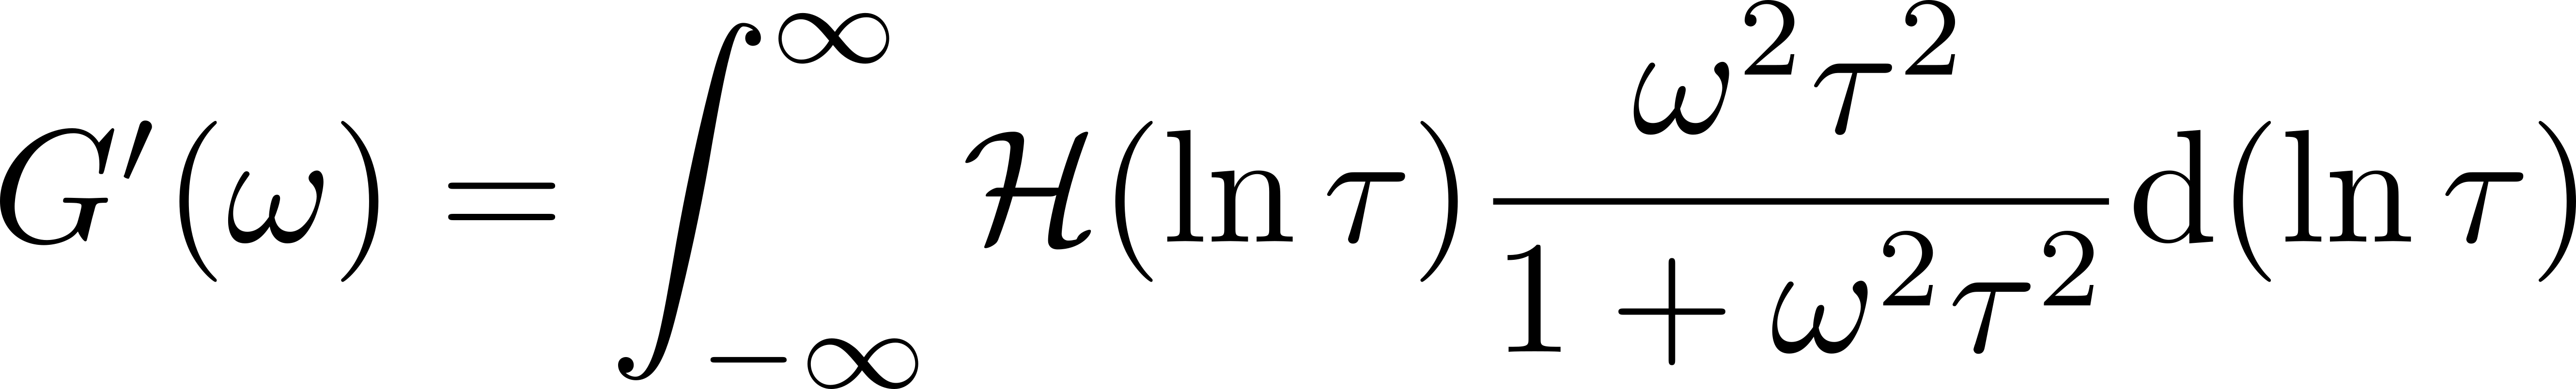
\includegraphics{fig/fig_1/ややこしい数式.png}
\caption{w:15cm}
\end{figure}

\end{block}

\end{frame}

\begin{frame}

\begin{block}{油断するとよくわからない(逃げ言葉?)}

\begin{itemize}

\item
  「応力集中が粘弾性により緩和します。」
\item
  「非ニュートン流体の特徴的な流動を設計しなければいけない。」
\item
  「チクソ性の高い液体は液だれしにくい。」
\item
  「のど越しのいいビールは筋電図の低周波成分を抑制できるものである。」
\end{itemize}

{分かったような、でもなんだかよく考えると、ヤッパリ良く判らない言葉。}

\end{block}

\end{frame}

\begin{frame}

\begin{block}{混乱しやすいもう一つの原因}

\begin{itemize}

\item
  レオロジーの対象は非常に幅広い

  \begin{itemize}
  
  \item
    人間の心地よさをレオロジー的感覚で評価

    \begin{itemize}
    
    \item
      「ナタデココ」
    \item
      肌触りのよい下着
    \end{itemize}
  \item
    機能設計にレオロジーを利用

    \begin{itemize}
    
    \item
      ショックのない運動靴
    \item
      塗り易くて液だれしない塗料
    \end{itemize}
  \end{itemize}
\end{itemize}

{微妙に使っている言葉が異なり混乱しやすい。}

\end{block}

\end{frame}

\begin{frame}

\begin{block}{よくある状態}

\begin{itemize}

\item
  ありがちな両極端

  \begin{itemize}
  
  \item
    脳筋\\
    とにかく測れ
  \item
    頭でっかち\\
    理屈ばかりで手が動かない
  \end{itemize}
\item
  誰もが、最初は素人

  \begin{itemize}
  \item
    うまくやっている人の物まねが手っ取り早い
  \item
    でも、近くにいい先輩がいないときは?
  \item ~
    \subsection{新しい問題へのアプローチは?}
  \end{itemize}
\end{itemize}

\end{block}

\begin{block}{理解へのアプローチ}

\end{block}

\end{frame}

\begin{frame}

\begin{block}{ヤッパリ分かりにくい}

\begin{itemize}

\item
  レオロジー技術

  \begin{itemize}
  
  \item
    非常に多様な切り口での議論

    \begin{itemize}
    
    \item
      食品、塗料、心地よさ、潤滑油、等々
    \end{itemize}
  \item
    それぞれの要素技術が異なる⇔内容が多岐
  \item
    一見複雑に見える。
  \end{itemize}
\item
  そのため、この分野に興味を持たれた初心者の方たちの中には、習得するのが大変そうだなと思われている方も多いのかもしれない。
\end{itemize}

\end{block}

\end{frame}

\begin{frame}{急がば回れ}

\end{frame}

\begin{frame}

\begin{block}{イメージで捉えてみては}

\begin{itemize}

\item
  イメージとして全体像をザックリと捕まえることができれば、理解は一気に容易になる。
\item
  「レオロジー」を、工学的に簡単に言えば、

  \begin{itemize}
  
  \item
    「物質」に、
  \item
    「刺激(変形、応力)を与えると」、
  \item
    「どうなるか(流れる、応力を発生)?」
  \end{itemize}
\item
  {大事なポイント:時間のことも考慮に入れる。}
\end{itemize}

\end{block}

\end{frame}

\begin{frame}

\begin{block}{「見える化」}

\begin{itemize}

\item
  「何をやりたいのか?」を常に意識しながら、

  \begin{itemize}
  
  \item
    因果関係をはっきりと

    \begin{itemize}
    
    \item
      因←原因\\
    \item
      果←結果
    \end{itemize}
  \item
    図として捉える

    \begin{itemize}
    
    \item
      複雑な実事象をできるだけ単純化
    \item
      一目で理解できるように
    \end{itemize}
  \end{itemize}
\end{itemize}

\end{block}

\end{frame}

\begin{frame}

\begin{block}{色々なモデル化}

例えば、東洋思想においての考え方

\begin{itemize}

\item
  単純化

  \begin{itemize}
  
  \item
    陰陽思想⇔二分化
  \item
    五行思想⇔分類
  \end{itemize}
\item
  組み合わせ

  \begin{itemize}
  
  \item
    陰陽五行
  \item
    八卦
  \end{itemize}
\end{itemize}

ギリシア思想でも似たようなもの

\end{block}

\end{frame}

\begin{frame}

\begin{block}{モデル化の適正な度合い}

\begin{itemize}

\item
  適度な深さで尤もらしく

  \begin{itemize}
  
  \item
    簡単すぎるものは例外が多い。
  \item
    複雑化しすぎても過適応

    \begin{itemize}
    
    \item
      n個のデータを、n次の関数でフィット\\
    \item
      個々の現象にだけ適応可能
    \item
      モデル化する意味がない
    \end{itemize}
  \end{itemize}
\item
  欲しいもの

  \begin{itemize}
  
  \item
    汎用的に使えるモデル
  \item
    尤もらしく、実験事実を説明できるもの
  \end{itemize}
\end{itemize}

\end{block}

\end{frame}

\begin{frame}

\begin{block}{本講座の進め方}

\end{block}

\end{frame}

\begin{frame}

\begin{block}{本講座の進め方}

以下のような点に気を付けて進めます。

\begin{itemize}

\item
  イメージしやすい、直感的な理解を目指す。

  \begin{itemize}
  
  \item
    全体を俯瞰した概念的な説明
  \item
    多様な切り口からの説明\\
  \end{itemize}
\item
  大事なことは何度か繰り返す。

  \begin{itemize}
  
  \item
    一度ではわかりにくいかも。
  \item
    似たような内容を、ちょっと違う言葉で。
  \end{itemize}
\item
  ゆっくり議論

  \begin{itemize}
  \item ~
    \subsection{\texorpdfstring{{理解し難いことはいつでも聞いて下さい。}}{理解し難いことはいつでも聞いて下さい。}}
  \end{itemize}
\end{itemize}

\end{block}

\begin{block}{「数式に頼らない」という意味}

\begin{itemize}

\item
  「天下りの数式展開」は無駄。

  \begin{itemize}
  
  \item
    意味の理解できない数式は無意味
  \item
    たいてい、思考停止を招くだけ。
  \end{itemize}
\item
  でも、状態をイメージするためには、数学的な感覚は有効

  \begin{itemize}
  
  \item
    数学(算数?)的な事項の復習も。
  \item
    物理的なイメージを数学とつなげて理解
  \end{itemize}
\item
  私に分かり易い表現があなたに有効とは限らないので数式の表すものを議論しましょう。

  \begin{itemize}
  
  \item
    {理解し難いことはいつでも聞いて下さい。}
  \end{itemize}
\end{itemize}

\end{block}

\end{frame}

\begin{frame}

\begin{block}{参考書}

\begin{itemize}

\item
  レオロジー関連

  \begin{itemize}
  
  \item
    \href{https://www.amazon.co.jp/\%E3\%83\%AC\%E3\%82\%AA\%E3\%83\%AD\%E3\%82\%B8\%E3\%83\%BC\%E5\%9F\%BA\%E7\%A4\%8E\%E8\%AB\%96-\%E6\%9D\%91\%E4\%B8\%8A-\%E8\%AC\%99\%E5\%90\%89/dp/4782825315}{レオロジー基礎論:村上鎌吉}
  \item
    \href{https://www.amazon.co.jp/\%E3\%81\%8A\%E3\%82\%82\%E3\%81\%97\%E3\%82\%8D\%E3\%83\%AC\%E3\%82\%AA\%E3\%83\%AD\%E3\%82\%B8\%E3\%83\%BC-\%E2\%80\%95\%E3\%81\%A9\%E3\%82\%8D\%E3\%81\%A9\%E3\%82\%8D\%E3\%80\%81\%E3\%81\%90\%E3\%81\%AB\%E3\%82\%83\%E3\%81\%90\%E3\%81\%AB\%E3\%82\%83\%E7\%89\%A9\%E8\%B3\%AA\%E3\%81\%AE\%E7\%A7\%91\%E5\%AD\%A6-\%E7\%9F\%A5\%E3\%82\%8A\%E3\%81\%9F\%E3\%81\%84-\%E3\%82\%B5\%E3\%82\%A4\%E3\%82\%A8\%E3\%83\%B3\%E3\%82\%B9-\%E5\%A2\%97\%E6\%B8\%95/dp/4774143103/ref=sr_1_fkmrnull_1?__mk_ja_JP=\%E3\%82\%AB\%E3\%82\%BF\%E3\%82\%AB\%E3\%83\%8A\&crid=3NKUKEKY9NBUV\&keywords=\%E3\%81\%8A\%E3\%82\%82\%E3\%81\%97\%E3\%82\%8D\%E3\%83\%AC\%E3\%82\%AA\%E3\%83\%AD\%E3\%82\%B8\%E3\%83\%BC\&qid=1557628414\&s=gateway\&sprefix=\%E3\%81\%8A\%E3\%82\%82\%E3\%81\%97\%E3\%82\%8D\%E3\%82\%8C\%E3\%81\%8A\%2Cstripbooks\%2C250\&sr=8-1-fkmrnull}{おもしろレオロジー:増渕雄一}
  \item
    \href{https://www.amazon.co.jp/\%E3\%83\%AC\%E3\%82\%AA\%E3\%83\%AD\%E3\%82\%B8\%E3\%83\%BC\%E3\%81\%AE\%E4\%B8\%96\%E7\%95\%8C\%E2\%80\%95\%E5\%9F\%BA\%E6\%9C\%AC\%E6\%A6\%82\%E5\%BF\%B5\%E3\%81\%8B\%E3\%82\%89\%E7\%89\%B9\%E6\%80\%A7\%E3\%83\%BB\%E6\%A7\%8B\%E9\%80\%A0\%E3\%83\%BB\%E8\%A6\%B3\%E6\%B8\%AC\%E6\%B3\%95\%E3\%81\%BE\%E3\%81\%A7-\%E5\%B0\%BE\%E5\%B4\%8E-\%E9\%82\%A6\%E5\%AE\%8F/dp/4769341814/ref=pd_sbs_14_3/355-3703731-4533608?_encoding=UTF8\&pd_rd_i=4769341814\&pd_rd_r=58a50bf2-745e-11e9-8b82-99118fb491a2\&pd_rd_w=9I9I8\&pd_rd_wg=Z5H9Q\&pf_rd_p=ad2ea29d-ea11-483c-9db2-6b5875bb9b73\&pf_rd_r=DKRCWCM52WW6JDE1YE82\&psc=1\&refRID=DKRCWCM52WW6JDE1YE82}{レオロジーの世界:尾崎邦弘}
  \item
    新講座・レオロジー:日本レオロジー学会
  \end{itemize}
\item
  その他

  \begin{itemize}
  
  \item
    オイラーの贈物:吉田武
  \end{itemize}
\end{itemize}

\end{block}

\end{frame}

\begin{frame}

\begin{block}{スライド画面表示だけに頼らない理由}

\begin{itemize}

\item
  一枚の画像の中の情報の重要性は分かり難い

  \begin{itemize}
  
  \item
    \href{https://gigazine.net/news/20190506-powerpoint-slide-killed-seven-people/}{「7人の命を奪ったPowerPointのスライド発表」とは?
    - GIGAZINE}
  \item
    一枚ごとの情報を少なく。
  \end{itemize}
\item
  イメージをはっきり持つためには、ただ聞いているのではなく議論に参加。

  \begin{itemize}
  
  \item
    \href{https://gigazine.net/news/20140413-switch-to-whiteboard/}{なぜフェルミ国立加速器研究所はPowerPointを禁止し黒板を使用するのか?
    - GIGAZINE}
  \end{itemize}
\item
  {理解し難いことはいつでも聞いて下さい。}
\end{itemize}

\end{block}

\end{frame}

\begin{frame}

aaa

試験用に作成中

Column 1 Contentここに書けばいいのだ。

\begin{figure}
\centering
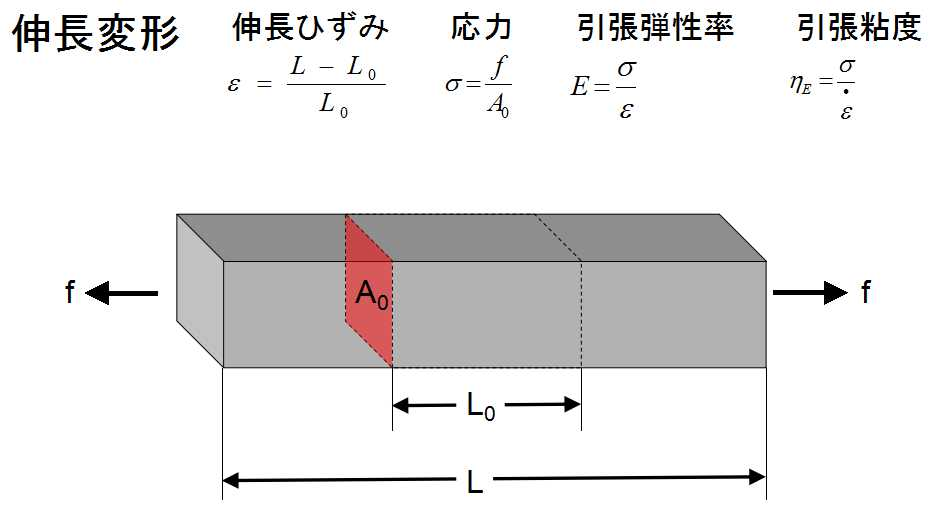
\includegraphics{単純な伸長変形のモデル.jpg}
\caption{w:10cm}
\end{figure}

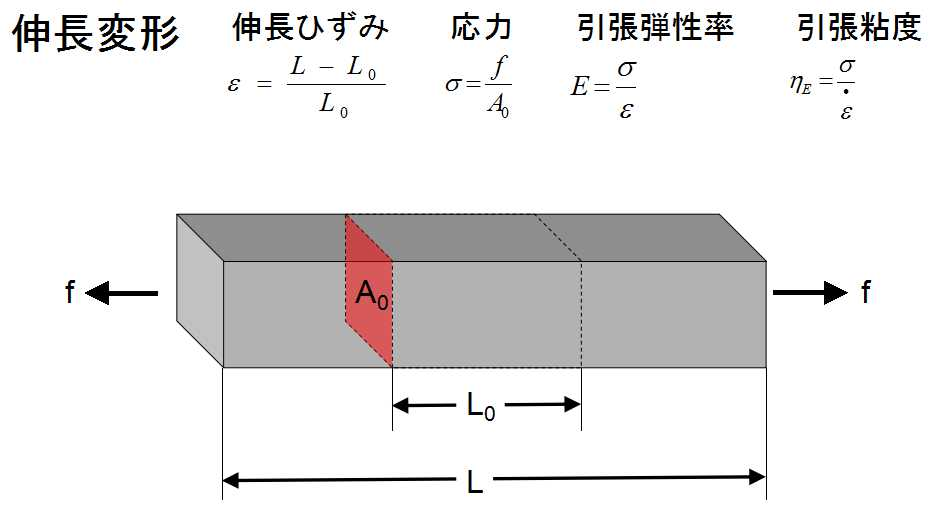
\includegraphics{単純な伸長変形のモデル.jpg} Column 2 Content

Column 1 Contentここに書けばいいのだ。

vvv

\end{frame}

\begin{frame}

\end{frame}

\begin{frame}[fragile]{Fragmented list}

\begin{itemize}
\item
  One

  \begin{itemize}
  
  \item
    sss
  \item
    fff

    \begin{itemize}
    
    \item
      hhh
    \end{itemize}
  \end{itemize}
\item
  Two

  \begin{itemize}
  
  \item
    a
  \item
    b
  \end{itemize}
\item ~
  \subsection{Three}
\end{itemize}

Add underscore prefix \texttt{\_} to the name of local directives.

\end{frame}

\begin{frame}{ppp}

\begin{block}{\#\# GGG}

The second page would not apply setting of directives.

\end{block}

\end{frame}

\begin{frame}{Ordered list}

\begin{enumerate}

\item
  One
\item
  Two
\item
  Three
\end{enumerate}

\end{frame}

\begin{frame}{Fragmented list}

\begin{enumerate}
[1)]

\item
  One
\item
  Two
\item
  Three
\end{enumerate}

\end{frame}
